\chapter{Circles and Angles}
\paragraph{} On the tenth day, Bessie had an issue: Farmer John was bored and kept causing trouble on the farm. Rather than letting her and the other cows graze, he was trying to cut down their grass. To keep him entertained and away from the grass, Bessie decided to create crop circles in the corn field.
\paragraph{} "Duckie!" she called. "Want to help make some crop circles?"
\paragraph{} "Sure! I think it will be great for helping my wing recover!" Duckie replied.
\vfill.
\pagebreak
\subchapter{Angles}
{Bessie and Duckie came up with a plan to draw their circles. They decided that Duckie would fly around Bessie, staying exactly $\mathbf{7} m$ away from Bessie at each point. To make sure Duckie is exactly the same distance, Bessie would spin around and look at him at any given point. Bessie knows she will get dizzy if she spins too much, so decides to keep track of how much she has turned at any moment.}
{}
{The number of meters between the Duckie and Bessie is called r, or the “radius”. When Duckie has flown r meters around Bessie, the amount Bessie has turned is a “radian”.}
{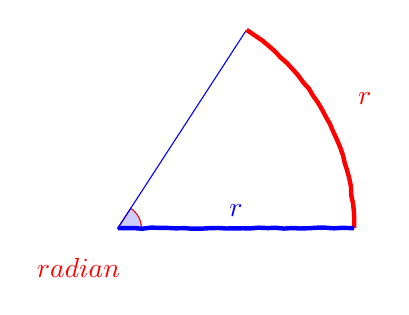
\begin{tikzpicture}
     \filldraw[fill=blue!20,draw=red] (0,0) -- (3mm,0mm)
    arc [start angle=0, end angle=57, radius=3mm] -- cycle;
    \node[red] at (-0.5,-0.5) {$radian$};
    \draw[blue] (3,0) -- ++(0+180:3) -- +(57:3);
    \draw[red, decorate, decoration={random steps,segment length=3pt,amplitude=0.2pt}, ultra thick] (3,0) arc[start angle=0, end angle=57, radius=3] node [midway,above,xshift=0.5cm] {$r$};
    \draw[blue, decorate, decoration={random steps,segment length=3pt,amplitude=0.2pt}, ultra thick] (0,0) -- (3,0) node [midway,above] {$r$};
\end{tikzpicture}}
\subchapter{Drawing a single Circle}
{Bessie and Duckie began to draw the first circle, but ran into an issue. She didn't know when to stop spinning! How many radians does Bessie have to turn so that Duckie makes a full circle (and she looks in the same place she started)?}
{}
{When Duckie has flown a full circle around Bessie and Bessie was looking in the same direction where she started, she had turned around $2\ast\pi$ radians. This amount Bessie turned cannot be written as a fraction, and so is called “irrational”. This specific irrational number has the name “pi”. 
\paragraph{} For convenience, approximate $\pi$ to be $\frac{22}{7}$ (the actual value of pi is slightly smaller).}
{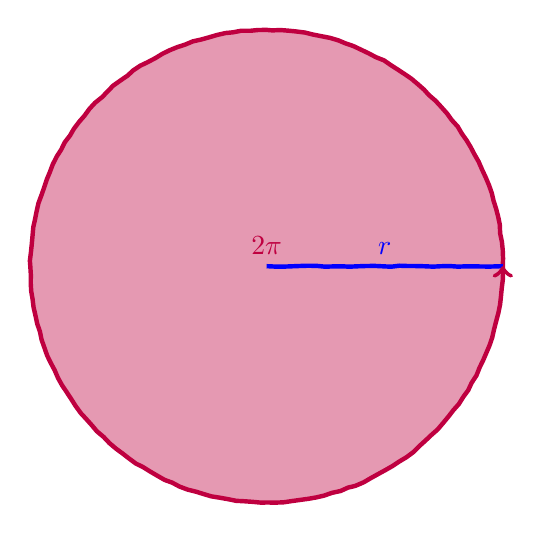
\begin{tikzpicture}
    \draw[purple, decorate, decoration={random steps,segment length=3pt,amplitude=0.2pt}, ultra thick,fill=purple!40!white] (0,0) circle (3) node [above] {$2\pi$};
    \draw[blue, decorate, decoration={random steps,segment length=3pt,amplitude=0.2pt}, ultra thick] (0,0) -- (3,0) node [midway, above] {$r$};
    \draw[->,purple, decorate, decoration={random steps,segment length=3pt,amplitude=0.2pt}, ultra thick] (3,0)--(3,0);
\end{tikzpicture}}
\subchapter{Perimeter of a Circle}
{After some effort calculating, Duckie drew one full circle around Bessie. But, because of his injured wing, he began to feel a bit tired. He decided that in the full day, he would only fly a little so that his wing could recover properly. How much has Duckie flown?}
{For every radian Bessie turned, Duckie flew $7 m$. Because Bessie turned $2\ast \pi$ radians, Duckie have must turned $7\ast 2\ast\pi) m$. Using $\frac{22}{7}$ as $\pi$, we get $\frac{2\ast 22\ast 7}{7}=\frac{2\ast 22}{\ast 1}=44 m$}
{The perimeter of a circle is always $2\ast\pi\ast r$, where r is radius of the circle.}
{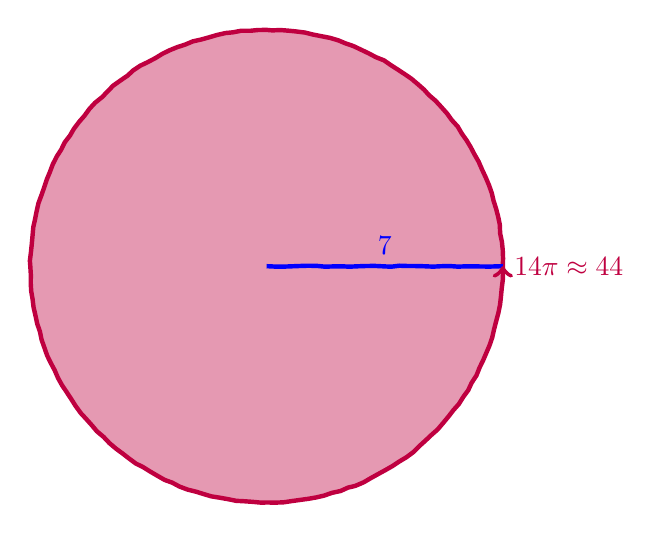
\begin{tikzpicture}
    \draw[purple, decorate, decoration={random steps,segment length=3pt,amplitude=0.2pt}, ultra thick,fill=purple!40!white] (0,0) circle (3) node [right,xshift=3cm] {$14\pi\linebreak\approx 44$};
    \draw[blue, decorate, decoration={random steps,segment length=3pt,amplitude=0.2pt}, ultra thick] (0,0) -- (3,0) node [midway, above] {$7$};
    \draw[->,purple, decorate, decoration={random steps,segment length=3pt,amplitude=0.2pt}, ultra thick] (3,0)--(3,0);
\end{tikzpicture}}
\subchapter{Trigonometric Functions}
{After resting for a few minutes, Duckie and Bessie started drawing their next circle. They decided that, to help give Farmer John some contrast, they would make it have a radius of 1. While creating the circle, tragedy struck! Duckie lost track of where he was! He sees that Bessie turned $\frac{\pi}{4}$ radians. What is Duckie's vertical position? What is Duckie's horizontal position?}
{When Bessie rotated $\frac{\pi}{2}$ radians, Duckie's vertical position and horizontal positions are $\frac{\pi}{2}$.}
{Take a line of length 1. As we rotate the line, we can see it has both a height and a width. When it starts, it has width but not height. When it rotates $\frac{\pi}{2}$ radians it has height but not width. When x is the angle rotated, the width at each angle (or the adjacent side/the diagonal side) is $cos(x)$. The height at each angle (or the opposite side/the diagonal side) is $sin(x)$. The ratio between these, $\frac{sin(x)}{cos(x)}$ is called $tan(x)$.\footnote{These functions, and other trigonometric functions can be viewed here. \url{https://visualize-it.github.io/trig_functions/simulation.html}}}
{\begin{tikzpicture}[scale=3]
    %\draw[step=.5cm,gray,very thin] (-1.4,-1.4) grid (1.4,1.4);
    \filldraw[fill=blue!20,draw=red] (0,0) -- (3mm,0mm)
    arc [start angle=0, end angle=45, radius=3mm] -- cycle;
    \node[red] at (15:2mm) {$\alpha$};
    \draw[->] (-1.5,0) -- (1.5,0) coordinate (x axis)node[right]{$Horizontal$};
    \draw[->] (0,-1.5) -- (0,1.5) coordinate (y axis)node[above]{$Vertical$};
    \draw (0,0) circle [radius=1cm];
    \draw[ultra thick,orange, decorate, decoration={random steps,segment length=3pt,amplitude=0.2pt}]
    (45:1cm) -- node[left=1pt,fill=white] {$\sin \alpha$} (45:1cm |- x axis);
    \draw[ultra thick,blue, decorate, decoration={random steps,segment length=3pt,amplitude=0.2pt}]
    (45:1cm |- x axis) -- node[below=2pt,fill=white] {$\cos \alpha$} (0,0);
    \path [name path=upward line, decorate, decoration={random steps,segment length=3pt,amplitude=0.2pt}] (1,0) -- (1,1);
    \path [name path=sloped line] (0,0) -- (45:1.5cm);
    \draw [name intersections={of=upward line and sloped line, by=t}, decorate, decoration={random steps,segment length=3pt,amplitude=0.2pt}]
    [ultra thick,red, decorate, decoration={random steps,segment length=3pt,amplitude=0.2pt}] (1,0) -- node [right=1pt,fill=white]
    {$\displaystyle \tan \alpha$} (t);
    \draw (0,0) -- (t);
    \foreach \x/\xtext in {-1, -0.5/-\frac{1}{2}, 1}
    \draw (\x cm,1pt) -- (\x cm,-1pt) node[anchor=north,fill=white] {$\xtext$};
    \foreach \y/\ytext in {-1, -0.5/-\frac{1}{2}, 0.5/\frac{1}{2}, 1}
    \draw (1pt,\y cm) -- (-1pt,\y cm) node[anchor=east,fill=white] {$\ytext$};
\end{tikzpicture}}
\subchapter{Trigonometric Identities}
{Duckie, tired, but with a healed wing, sat down. He and Bessie were ready to take the day off, and he was ready to start flying the next day. Güs, who had been planting grass, walked over to them. 
\paragraph{} "Hey Guys! How was your work in the cornfield?"
\paragraph{} "It was pretty good!" Bessie replied. "We were drawing circles for Farmer John while you planted grass."
\paragraph{} Güs looked at Bessie in surprise. "That's what you were doing? I thought you were tracing the point of an arrow where the width\texttimes the width plus the height\texttimes the height equaled one!"
The trio looked at each other in confusion. Who is right?}
{They were all right! The width of the arrow is cos(x), and the height of the arrow is sin(x). Through Pythagorean Theorem, the length of the arrow must be 1, which is also the radius that Duckie flew.}
{$sin(x)\ast sin(x) + cos(x)\ast cos(x) = 1\ast 1 = 1$.}
{}